\documentclass[11pt,a4paper]{article}
\RequirePackage[margin=1in]{geometry}
\RequirePackage[T1]{fontenc}
\RequirePackage{lmodern}
\RequirePackage{amsmath,amssymb,bm}
\RequirePackage{graphicx}
\RequirePackage{booktabs,array,float}
\RequirePackage{siunitx}
\RequirePackage[font=small,labelfont=bf]{caption}
\RequirePackage{subcaption}
\RequirePackage{xcolor}
\RequirePackage{fancyhdr}
\RequirePackage{titlesec}
\RequirePackage{hyperref}
\hypersetup{colorlinks=true,linkcolor=black,urlcolor=blue,citecolor=black}
\sisetup{round-mode=places,round-precision=5,detect-all}
\setlength{\headheight}{14pt}
\setlength{\parindent}{15pt}
\setlength{\parskip}{0pt}
\setlength{\emergencystretch}{2em}
\renewcommand{\arraystretch}{1.12}
\titleformat{\section}{\normalfont\Large\bfseries}{\thesection}{0.7em}{}
\titlespacing*{\section}{0pt}{1.2ex plus .2ex}{0.7ex}
\titleformat{\subsection}{\normalfont\large\bfseries}{\thesubsection}{0.7em}{}
\titlespacing*{\subsection}{0pt}{1.0ex plus .2ex}{0.45ex}
\fancyhf{}
\fancyhead[L]{CE587 Homework 1}
\fancyhead[R]{Imran Shahriar - 2735835}
\renewcommand{\headrulewidth}{0.4pt}
\fancyfoot[C]{\thepage}
\fancypagestyle{plain}{%
  \fancyhf{}
  \fancyhead[L]{CE587 Homework 1}
  \fancyhead[R]{Imran Shahriar - 2735835}
  \renewcommand{\headrulewidth}{0.4pt}
  \fancyfoot[C]{\thepage}}
\pagestyle{fancy}


\usepackage{pdflscape}
\graphicspath{{./}{figures/}}
\newlength{\worksheetlandscapewidth}
\newcommand{\worksheetportrait}[3]{%
  \subsubsection*{#1}
  \vspace{0.25em}
  \begin{center}
    \makebox[\textwidth][c]{\includegraphics[height=0.79\textheight,keepaspectratio]{#2}}\par
    \vspace{0.35em}
    \captionsetup{hypcap=false}
    \captionof{figure}{#3}
  \end{center}}
\newcommand{\worksheetlandscape}[3]{%
  \setlength{\worksheetlandscapewidth}{\dimexpr\textheight-18pt\relax}%
  \begin{landscape}
    \thispagestyle{empty}
    \begin{minipage}[t][\textwidth][s]{\worksheetlandscapewidth}
      \subsubsection*{#1}
      \vspace{0.25em}
      \centering
      \includegraphics[width=0.96\linewidth,keepaspectratio]{#2}\par
      \vspace{0.35em}
      \captionsetup{hypcap=false}
      \captionof{figure}{#3}\par
      \vfill
      \makebox[\linewidth][c]{\thepage}
    \end{minipage}
  \end{landscape}}
\begin{document}
\hypersetup{pageanchor=false}
\begin{titlepage}
  \thispagestyle{empty}
  \begin{flushright}{\large\today\par}\end{flushright}
  \vspace*{0.5cm}
  \begin{center}
    
\includegraphics[width=0.42\textwidth]{metu_logo.jpg}\par
    \vspace{0.7cm}
    {\huge CE587 Homework 1\par}
    \vspace{0.3cm}
    {\Large Structural Optimization\par}
    \vspace{0.45cm}
    {\Large Fall Semester 2026--2027\par}
  \end{center}
  \vspace{1.0cm}
  \noindent
  \begin{minipage}[t]{0.48\textwidth}
    \raggedright
    {\Large\textbf{Submitted By}\par}
    \vspace{0.3cm}
    {\large Imran Shahriar\par}
    \vspace{0.2cm}
    {\large 2735835\par}
    \vspace{0.2cm}
    {\large MSc. in Structural Engineering\par}
  \end{minipage}\hfill
  \begin{minipage}[t]{0.48\textwidth}
    \raggedleft
    {\Large\textbf{Submitted To}\par}
    \vspace{0.3cm}
    {\large Prof. Dr. O\u{g}uzhan Hasan\c{c}ebi\par}
    \vspace{0.2cm}
    {\large Department of Civil Engineering\par}
    \vspace{0.2cm}
    {\large Middle East Technical University\par}
  \end{minipage}
  \vfill
\end{titlepage}
\hypersetup{pageanchor=true}
\setcounter{page}{1}

\section{Question 1 --- Hollow circular beam-column}
\subsection{Mathematical formulation (part a)}
A uniform thin-walled circular member of length $L=3$ m is designed for an axial load $P=50$ kN and self-weight. The axial-stress case and the self-weight deflection case are evaluated separately, as prescribed. The material data are $E=210$ GPa, $\rho=7800$ kg/m$^3$, allowable stress $\sigma_a=250$ MPa and $g=9.80$ m/s$^2$. The design bounds are $0.02\le R\le0.20$ m and $0.001\le t\le0.010$ m.

\paragraph{Design variables.} $\mathbf{x}_1=[R,t]^T$.

Using the thin-wall expressions supplied for the model,
\begin{align}
 A&=2\pi Rt, & I&=\pi R^3t, & w&=\rho gA,\\
 \sigma&=\frac{P}{A}, & \min_{R,t}\ m(R,t)&=\rho LA=2\pi\rho LRt.\label{eq:q1model}
\end{align}
The assignment gives $\delta=5wL^4/(384EI)$. Substituting $A$, $I$ and $w$ yields
\begin{equation}
 \delta=\frac{5\rho g(2\pi Rt)L^4}{384E\pi R^3t}
 =\frac{5\rho gL^4}{192ER^2}.
 \label{eq:q1deflection}
\end{equation}
The thickness cancels because self-weight and flexural stiffness both vary linearly with $t$. With $\delta_a=0.001L=3$ mm, the normalized constraints $g_i\le0$ are
\begin{align}
g_1&=\frac{P}{2\pi Rt\sigma_a}-1,&
g_2&=\frac{5\rho gL^4}{192ER^2\delta_a}-1,\\
g_3&=\frac{R}{20t}-1,&g_4&=\frac{0.02}{R}-1,\\
g_5&=\frac{R}{0.20}-1,&g_6&=\frac{0.001}{t}-1,\\
g_7&=\frac{t}{0.010}-1.&&\label{eq:q1constraints}
\end{align}
\paragraph{Objective function.} $\min_{\mathbf{x}_1} f_1(\mathbf{x}_1)=\rho L A=2\pi\rho LRt$.

\paragraph{Constraints.} The normalized inequalities are $g_i(\mathbf{x}_1)\le0$ for $i=1,\ldots,7$, as defined in (\ref{eq:q1constraints}). The lower bounds keep area and inertia positive. No additional stability or manufacturing limit is imposed.

\subsection{Graphical solution (part b)}
For graphing, use centimetres. The axial-stress boundary is $Rt=1/\pi$ cm$^2$, or $t=1/(\pi R)$, and the radius-to-thickness boundary is $t=R/20$. The deflection requirement gives $R\ge1.5998$ cm. Since the assigned lower radius is 2 cm, deflection is redundant; at $R=2$ cm, $\delta=1.920$ mm, below 3 mm. The feasible region lies above
\begin{equation}
 t_c(R)=\max\left\{0.1,\frac{1}{\pi R},\frac{R}{20}\right\},\qquad 2\le R\le20\ \mathrm{cm},
 \label{eq:q1ccs}
\end{equation}
and below $t=1$ cm. The dashed curve is the composite constraint surface (CCS). Figure~\ref{fig:q1zoom} focuses on the feasible corner so the full optimal segment and its representative endpoint can be distinguished. The 4.68, 5, 6 and 8 kg contours are shown.

\begin{figure}[H]
 \centering
 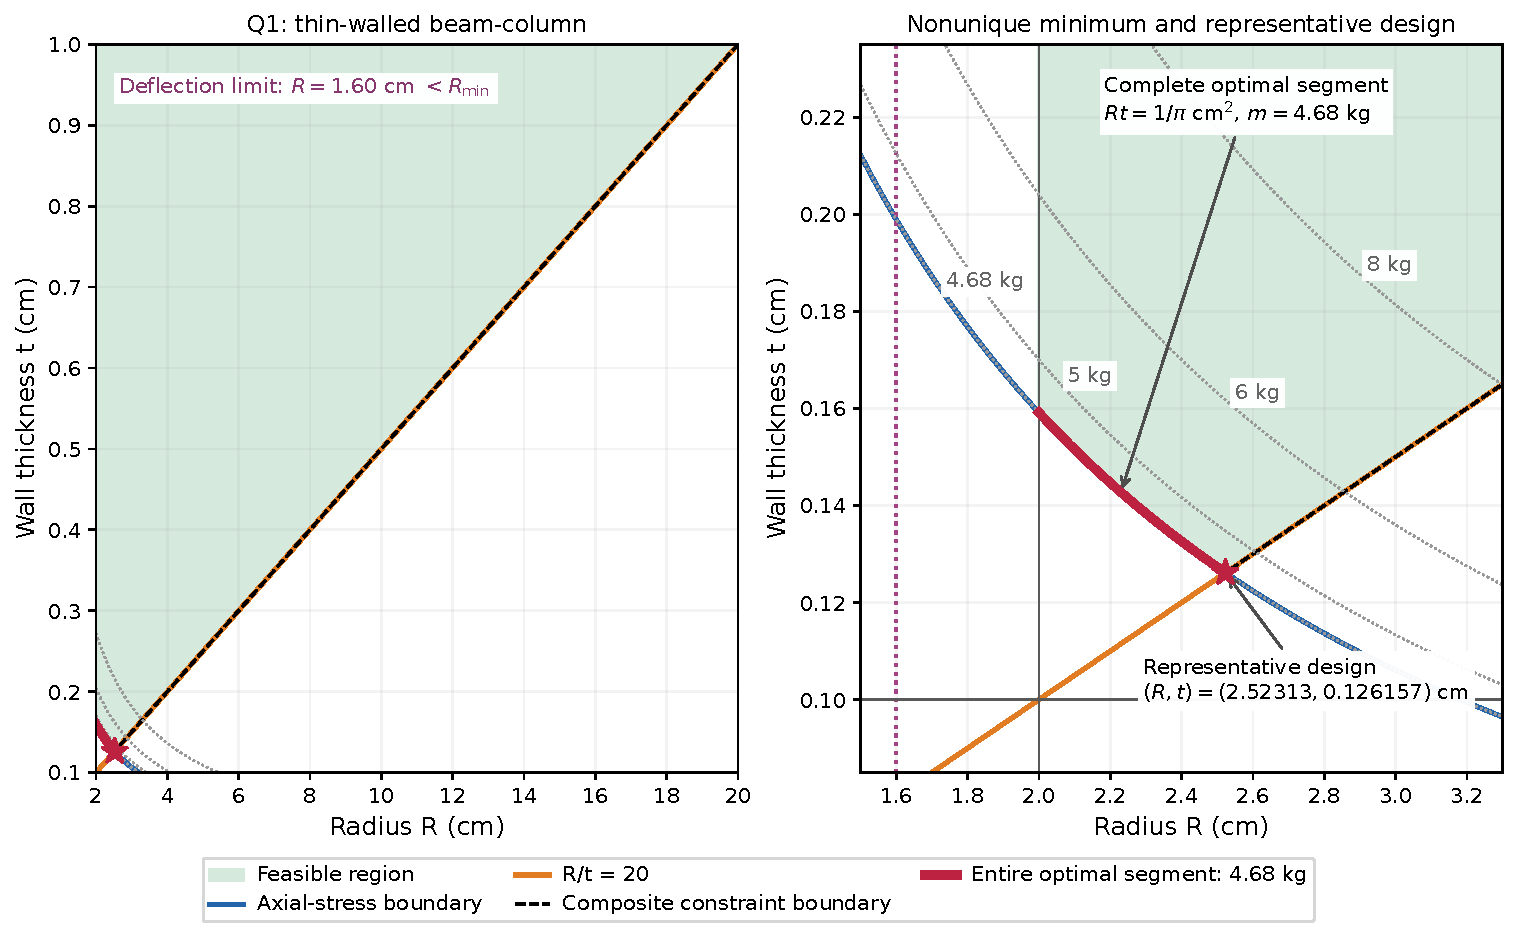
\includegraphics[width=0.98\textwidth]{figures/submission/q1_graphical.pdf}
 \caption{Q1 full design domain (left, $2\le R\le20$ cm and $0.1\le t\le1$ cm) and close-up of the optimum (right). Both panels show the feasible region, constraint boundaries, CCS and mass contours; the red curve is the complete minimum-mass set and the star marks its representative endpoint.}
 \label{fig:q1zoom}
\end{figure}

Since axial stress requires $A\ge P/\sigma_a$, every feasible design satisfies
\begin{equation}
 m=\rho LA\ge\rho L\frac{P}{\sigma_a}=4.680\ \mathrm{kg}.
 \label{eq:q1lowerbound}
\end{equation}
Equality holds when $Rt=1/\pi$ cm$^2$. Intersecting this curve with $R/t\le20$ and the radius and thickness bounds gives the complete optimal set
\begin{equation}
 \boxed{2.000\le R\le\sqrt{20/\pi}=2.52313\ \mathrm{cm},\qquad t=\frac{1}{\pi R}\ \mathrm{cm}.}
 \label{eq:q1optimalset}
\end{equation}
Thus the minimum is nonunique. The requested representative is the right endpoint, $(R,t)=(2.52313,0.126157)$ cm, where axial stress and $R/t$ are active.

\clearpage
\subsection{Microsoft Excel Solver (part c)}
The workbook sheet \texttt{Q1\_BeamColumn} uses centimetres for the changing cells and converts to SI in its response formulas. It calculates area, inertia, distributed self-weight, stress, deflection, mass and normalized constraint residuals. The saved Solver model uses the settings in Table~\ref{tab:q1solver}.

\begin{table}[H]
\centering\small
\caption{Q1 Solver configuration and design checks.}\label{tab:q1solver}
\setlength{\tabcolsep}{4pt}\begin{tabular}{@{}>{\raggedright\arraybackslash}p{0.19\textwidth}>{\raggedright\arraybackslash}p{0.22\textwidth}>{\raggedright\arraybackslash}p{0.28\textwidth}>{\raggedright\arraybackslash}p{0.25\textwidth}@{}}\toprule
Solver setting & Cell reference & Configuration / value & Result at representative design\\\midrule
Objective & B4 & Minimize & $m=4.6800$ kg\\
Changing cells & B7:B8 & Radius and thickness (cm) & $R=2.52313$, $t=0.126157$ cm\\
Constraints & B29:B35 $\le$\newline C29:C35 & Normalized constraints & See checks below\\
Explicit bounds & G11:G14; B7:B8 & $2\le R\le20$, $0.1\le t\le1$ cm & Bounds inactive\\
Method & -- & GRG Nonlinear & Saved native Solver model\\
Precision / convergence & -- & $10^{-9}/10^{-9}$ & --\\
Iterations / time & -- & 1500 / 100 s & --\\
Scaling / derivatives & -- & Automatic / central & --\\
Initial design & B7:B8 & $R=3$ cm, $t=0.15$ cm & --\\
Axial stress & B29 & $\sigma/\sigma_a\le1$ & 250.000 MPa / 250 MPa, active\\
Self-weight deflection & B30 & $\delta/\delta_a\le1$ & 1.206 mm / 3 mm, inactive\\
R/t limit & B31 & $(R/t)/20\le1$ & 20.000 / 20, active\\
Radius / thickness bounds & B32:B35 & Lower and upper limits & Inactive\\
\bottomrule\end{tabular}
\end{table}

Excel returned $R=2.52313$ cm, $t=0.126157$ cm and $m=4.68000$ kg. The returned stress is within the configured Solver tolerance; the analytical point satisfies the limit exactly. Python gives the same dimensions and mass to the shown precision. Appendix~\ref{app:excel} presents the worksheet and actual Solver Parameters dialog for Question 1; Table~\ref{tab:q1solver} summarizes the settings.

\clearpage
\section{Question 2 --- Hollow circular cantilever}
\subsection{Mathematical formulation (part d)}
A cantilever of length $L=10$ m carries a tip force $P=14$ kN. The material density is $7850$ kg/m$^3$; the allowable bending and shear stresses are 165 MPa and 50 MPa.

\paragraph{Design variables.} $\mathbf{x}_2=[R_o,R_i]^T$, with $0\le R_i<R_o\le0.40$ m.

For an exact annular section,
\begin{align}
A&=\pi(R_o^2-R_i^2),& I&=\frac{\pi}{4}(R_o^4-R_i^4),\\
\sigma&=\frac{PLR_o}{I},&
\tau&=\frac{P(R_o^2+R_oR_i+R_i^2)}{3I},\\
\min\quad m(R_o,R_i)&=\rho LA.&&\label{eq:q2model}
\end{align}
\paragraph{Objective function.} $\min_{\mathbf{x}_2} f_2(\mathbf{x}_2)=\rho L A$ as given in (\ref{eq:q2model}).

\paragraph{Constraints.} With $r_{\max}=0.40$ m, the normalized stress and radius inequalities are $g_i(\mathbf{x}_2)\le0$ for $i=1,\ldots,5$; the strict geometric condition is $g_6(\mathbf{x}_2)<0$:
\begin{align}
g_1&=\sigma/(165\ \mathrm{MPa})-1,&g_2&=\tau/(50\ \mathrm{MPa})-1,\\
g_3&=R_o/r_{\max}-1,&g_4&=R_i/r_{\max}-1,\\
g_5&=-R_i/r_{\max},&g_6&=(R_i-R_o)/r_{\max}<0.&&\label{eq:q2constraints}
\end{align}
The last relation is strict in the mathematical model. The workbook uses a $10^{-8}$ m positive-thickness guard to keep Solver away from the singular zero-area section; it is a numerical safeguard, not a manufacturing requirement.

\subsection{Graphical solution (part e)}
At a fixed $R_o$, increasing $R_i$ reduces the area and mass, so the upper feasible boundary is set by the first bending or shear limit reached. The bending boundary is
\begin{equation}
R_{i,b}(R_o)=\left(R_o^4-CR_o\right)^{1/4},\qquad C=\frac{4PL}{\pi\sigma_b},\qquad R_o\ge C^{1/3},
\label{eq:q2bendboundary}
\end{equation}
and the shear boundary follows from $\tau(R_o,R_i)=\tau_a$. Figure~\ref{fig:q2} shows the feasible region, both stress boundaries, the excluded equal-radii line, the CCS and mass contours. Its close view places the outer-radius limit and the optimum at $R_o=40$ cm on the same edge.

\begin{figure}[H]
 \centering
 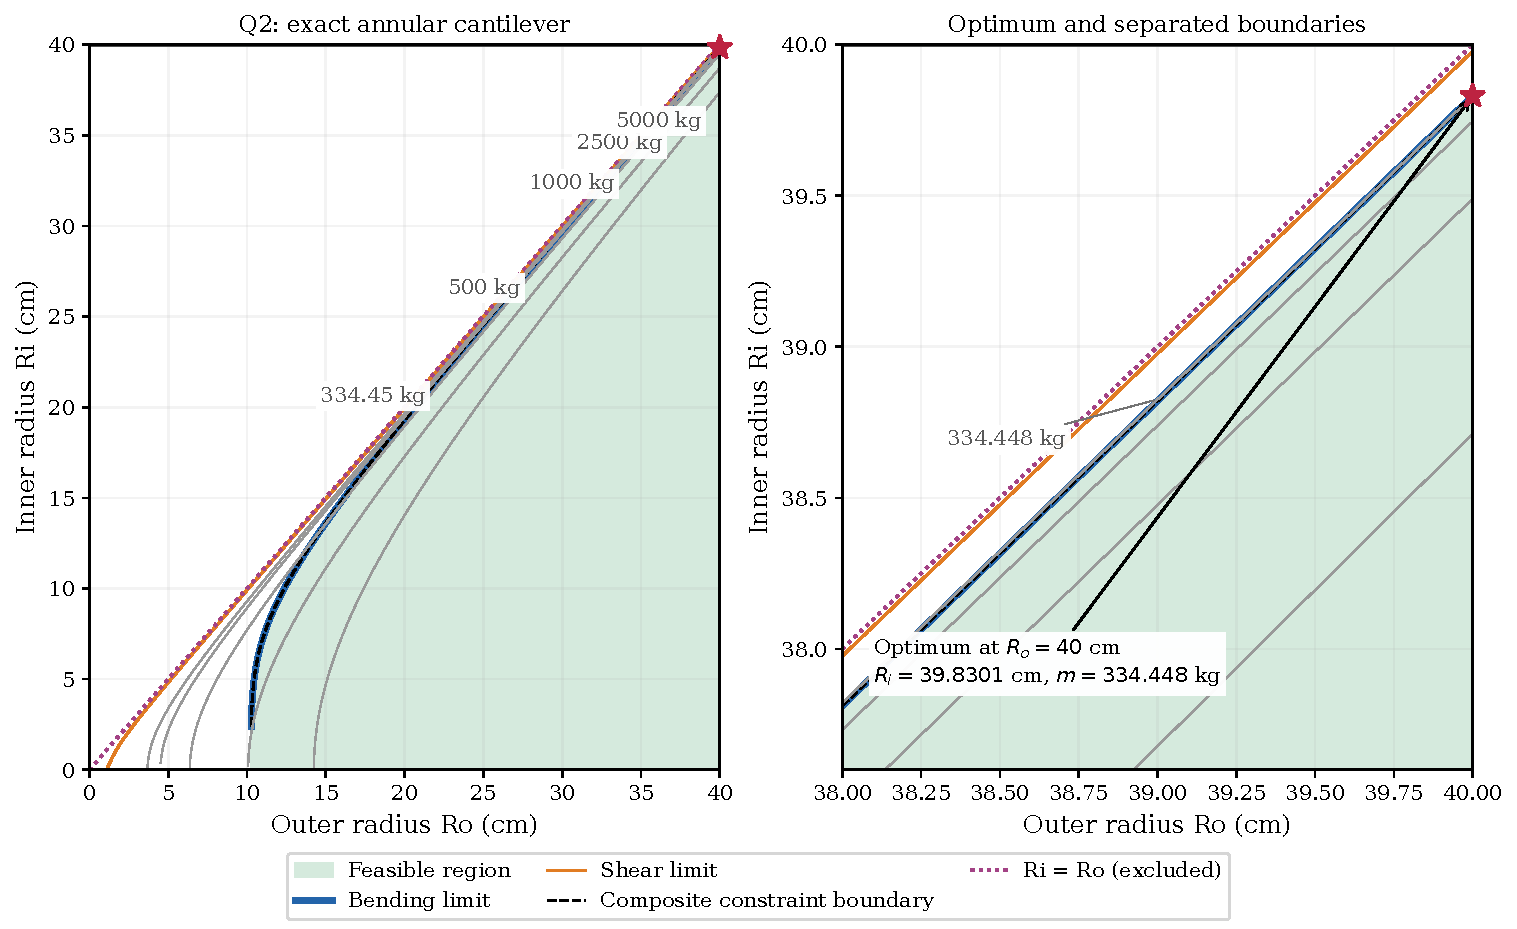
\includegraphics[width=0.98\textwidth]{figures/submission/q2_graphical.pdf}
 \caption{Q2 full design domain (left, $0\le R_o,R_i\le40$ cm) and close-up of the optimum (right). The bending and shear boundaries, excluded equal-radii line, CCS, mass contours and radius bound are shown in both panels. The star marks the optimum at $R_o=40$ cm.}
 \label{fig:q2}
\end{figure}

Shear is redundant for every bending-feasible section because
\begin{equation}
\frac{\tau}{\sigma}=\frac{R_o^2+R_oR_i+R_i^2}{3LR_o}\le\frac{R_o}{L}\le0.04,
\qquad \tau\le6.6\ \mathrm{MPa}<50\ \mathrm{MPa}.
\label{eq:q2shearproof}
\end{equation}
On the bending boundary the area can be written
\begin{equation}
A_b(R_o)=\frac{\pi C}{R_o+\sqrt{R_o^2-C/R_o}}.
\label{eq:q2areaboundary}
\end{equation}
The denominator increases with $R_o$, so the minimum mass decreases up to the assigned upper limit. The global optimum is therefore
\begin{equation}
\boxed{R_o^*=0.400000\ \mathrm{m},\quad R_i^*=0.398301\ \mathrm{m},\quad m^*=334.448\ \mathrm{kg}.}
\label{eq:q2opt}
\end{equation}
Bending and the outer-radius bound are active; shear is inactive. The wall is 1.69880 mm thick. This mathematical minimum would need local-buckling and fabrication checks in an actual design; those requirements are outside the assigned optimization model.

\subsection{Microsoft Excel Solver (part f)}
The \texttt{Q2\_Cantilever} sheet contains the annular properties, stresses, mass and constraint utilizations. Solver minimizes B4 by changing B7:B8. The stress rows use algebraically equivalent polynomial residuals, so trial evaluations remain finite near the geometric boundary; the reported design is checked against the original stress equations.

\begin{table}[H]
\centering\small
\caption{Q2 Solver configuration and final checks.}\label{tab:q2solver}
\setlength{\tabcolsep}{4pt}\begin{tabular}{@{}>{\raggedright\arraybackslash}p{0.19\textwidth}>{\raggedright\arraybackslash}p{0.22\textwidth}>{\raggedright\arraybackslash}p{0.28\textwidth}>{\raggedright\arraybackslash}p{0.25\textwidth}@{}}\toprule
Solver setting & Cell reference & Configuration / value & Result at optimum\\\midrule
Objective & B4 & Minimize & $m=334.448$ kg\\
Changing cells & B7:B8 & Outer and inner radii (cm) & $R_o=40.0000$, $R_i=39.8301$ cm\\
Stress constraints & B45:B46 $\le0$ & Smooth polynomial bending/shear residuals & Checked against stress equations\\
Radius constraints & B28:B31 $\le$\newline C28:C31; B7:B8 & Radius limits $0$--$40$ cm & $R_o=40$ cm, active\\
Geometry guard & B22 $\ge$ B16 & $\epsilon=10^{-8}$ m & $R_o-R_i=1.69880$ mm\\
Method & -- & GRG Nonlinear & Saved native Solver model\\
Precision / convergence & -- & $10^{-9}/10^{-9}$ & --\\
Iterations / time & -- & 2000 / 100 s & --\\
Scaling / derivatives & -- & Automatic / central & --\\
Initial design & B7:B8 & $R_o=30$ cm, $R_i=20$ cm & --\\
Bending stress & B26 & $\sigma/\sigma_b\le1$ & 165.000 MPa / 165 MPa, active\\
Shear stress & B27 & $\tau/\tau_a\le1$ & 6.572 MPa / 50 MPa, inactive\\
Mass & B4 & kg & 334.448 kg\\
\bottomrule\end{tabular}
\end{table}

Excel and Python agree within the saved Solver tolerance. Appendix~\ref{app:excel} presents the worksheet and actual Solver Parameters dialog for Question 2; Table~\ref{tab:q2solver} summarizes the settings.

\clearpage
\section{Question 3 --- Minimum-mass tripod}
\subsection{Mathematical formulation (part a)}
Three identical solid circular struts support an apex load $W=60$ kN over an equilateral base with side $B=120$ cm. The material is aluminum alloy 2014-T6 with $E=75$ GPa, $\rho=2800$ kg/m$^3$ and allowable compression stress $\sigma_a=150$ MPa. The safety factor is $FS=2$. Calculations use N and cm: $E=7.5\times10^6$ N/cm$^2$, $\rho=0.0028$ kg/cm$^3$, and $\sigma_a=15000$ N/cm$^2$.

\paragraph{Design variables.} $\mathbf{x}_3=[H,D]^T$, with $50\le H\le200$ cm and $0.5\le D\le10$ cm.

Each base vertex is a horizontal distance $B/\sqrt{3}$ from the centroid, so the strut length is $l=\sqrt{H^2+B^2/3}$. Symmetry cancels horizontal force components, while vertical equilibrium gives $3P(H/l)=W$. Thus
\begin{equation}
P=\frac{Wl}{3H},\quad A=\frac{\pi D^2}{4},\quad I=\frac{\pi D^4}{64},\quad
\sigma=\frac{P}{A},\quad P_{cr}=\frac{\pi^2EI}{l^2},\quad
\min\ m(H,D)=3\rho Al.
\label{eq:q3model}
\end{equation}
\paragraph{Objective function.} $\min_{\mathbf{x}_3}f_3(\mathbf{x}_3)=3\rho A l$ as given in (\ref{eq:q3model}).

\paragraph{Constraints.} The normalized inequalities are $g_i(\mathbf{x}_3)\le0$ for $i=1,\ldots,6$:
\begin{align}
g_1&=\frac{P}{A\sigma_a}-1,&g_2&=\frac{FS\,P}{P_{cr}}-1,\\
g_3&=\frac{50}{H}-1,&g_4&=\frac{H}{200}-1,\\
g_5&=\frac{0.5}{D}-1,&g_6&=\frac{D}{10}-1.&&\label{eq:q3constraints}
\end{align}
The prescribed strut length is used in Euler's formula and the safety factor is applied once.

\subsection{Graphical solution (part b)}
Solving the stress and buckling conditions for diameter gives
\begin{equation}
D_s(H)=\left(\frac{4Wl}{3\pi\sigma_aH}\right)^{1/2},\qquad
D_b(H)=\left(\frac{64FS\,Wl^3}{3\pi^3EH}\right)^{1/4},\qquad
D_c(H)=\max\{0.5,D_s,D_b\}.
\label{eq:q3boundaries}
\end{equation}
Figure~\ref{fig:q3} separates the compression-strength boundary from the Euler buckling boundary and shows their composite boundary with mass contours. In the assigned height range $D_b>D_s$; on the buckling boundary the maximum compression utilization is 0.247553 at $H=50$ cm. Thus buckling governs, while the compressive-strength constraint is inactive throughout.

\begin{figure}[H]
 \centering
 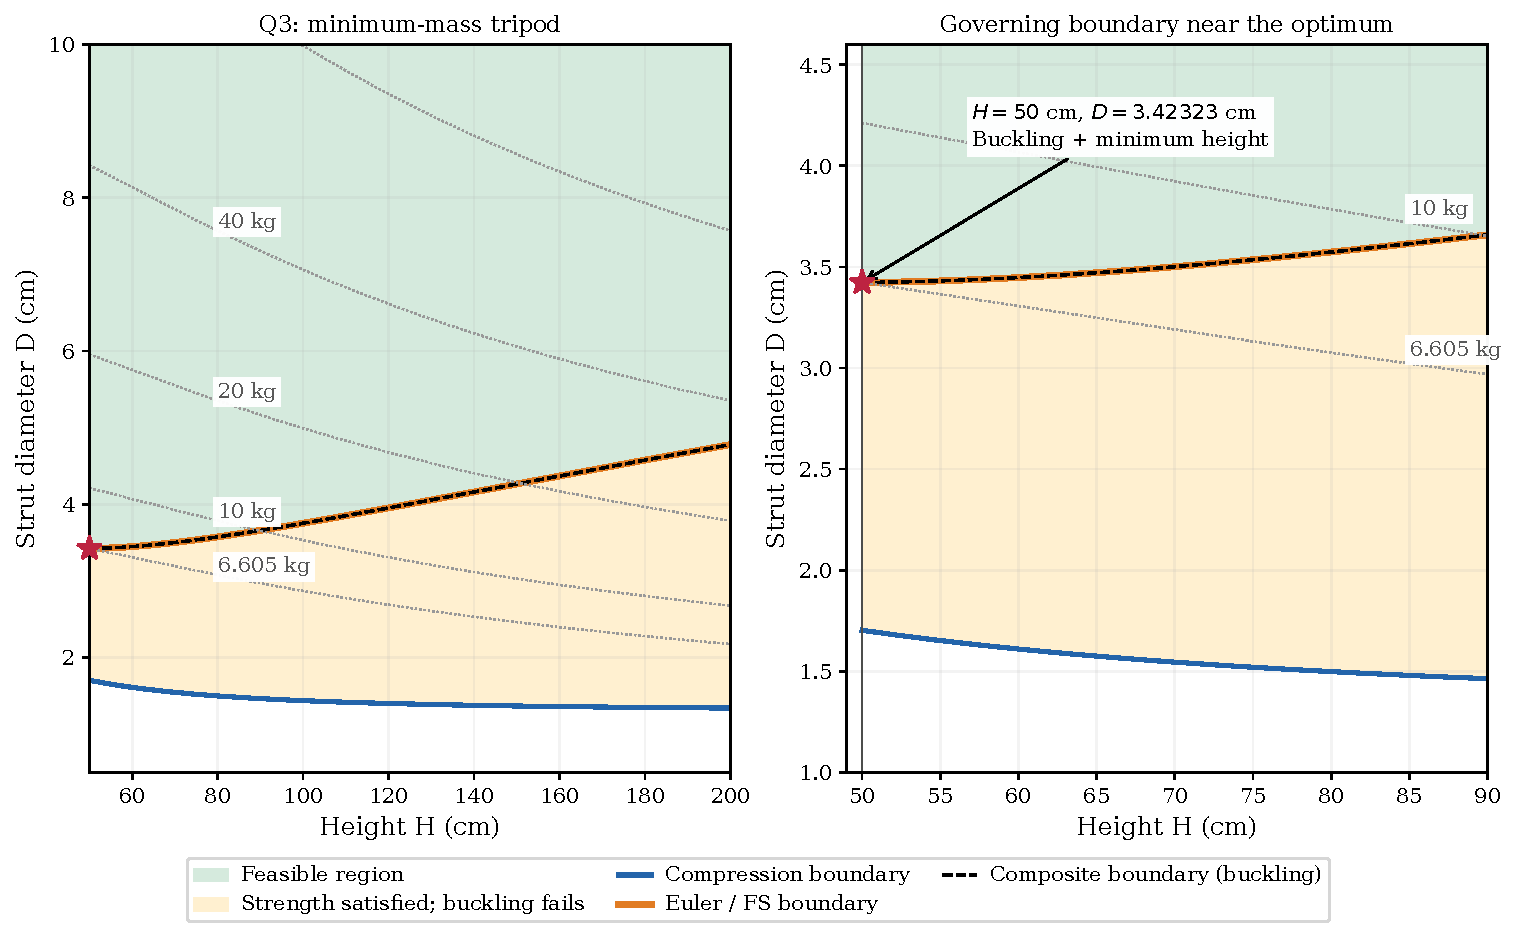
\includegraphics[width=0.98\textwidth]{figures/submission/q3_graphical.pdf}
 \caption{Q3 full design domain (left, $50\le H\le200$ cm and $0.5\le D\le10$ cm) and close-up near the minimum height (right). The compression-strength and Euler boundaries are distinct; the dashed CCS follows the buckling boundary. Amber indicates designs that pass strength but fail buckling. The star marks the optimum.}
 \label{fig:q3}
\end{figure}

For fixed $H$, mass increases with $D$, so the lightest feasible section lies at $D=D_b(H)$. Along that boundary $m_b(H)$ is proportional to $l^{5/2}H^{-1/2}$, and
\begin{equation}
\frac{d\log m_b}{dH}=\frac{4H^2-B^2/3}{2H(H^2+B^2/3)}>0\qquad(H\ge50\ \mathrm{cm}).
\label{eq:q3monotonic}
\end{equation}
The unconstrained stationary height $B/\sqrt{12}=34.641$ cm is below the permitted range. Therefore the minimum occurs at the lower height bound, with buckling active:
\begin{equation}
\boxed{H^*=50.0000\ \mathrm{cm},\quad D^*=3.42323\ \mathrm{cm},\quad m^*=6.60545\ \mathrm{kg}.}
\label{eq:q3opt}
\end{equation}

\subsection{Microsoft Excel Solver (part c)}
The \texttt{Q3\_Tripod} worksheet calculates strut geometry, equilibrium force, section properties, compression, Euler load, total mass and all six constraint utilizations. Solver minimizes B4 by changing B7:B8.

\begin{table}[H]
\centering\small
\caption{Q3 Solver configuration and final checks.}\label{tab:q3solver}
\setlength{\tabcolsep}{4pt}\begin{tabular}{@{}>{\raggedright\arraybackslash}p{0.19\textwidth}>{\raggedright\arraybackslash}p{0.22\textwidth}>{\raggedright\arraybackslash}p{0.28\textwidth}>{\raggedright\arraybackslash}p{0.25\textwidth}@{}}\toprule
Solver setting & Cell reference & Configuration / value & Result at optimum\\\midrule
Objective & B4 & Minimize & $m=6.60545$ kg\\
Changing cells & B7:B8 & Height and diameter (cm) & $H=50.0000$, $D=3.42323$ cm\\
Constraints & B26:B31 $\le$\newline C26:C31 & All six normalized constraints & --\\
Method & -- & GRG Nonlinear & Saved native Solver model\\
Precision / convergence & -- & $10^{-9}/10^{-9}$ & --\\
Iterations / time & -- & 2000 / 100 s & --\\
Scaling / derivatives & -- & Automatic / central & --\\
Initial design & B7:B8 & $H=100$ cm, $D=5$ cm & --\\
Compression stress & B26 & $\sigma/\sigma_a\le1$ & 37.133 MPa / 150 MPa, inactive\\
Euler buckling & B27 & $FS\,P/P_{cr}\le1$ & $P_{cr}=68.352$ kN $=2P$, active\\
Height lower bound & B28 & $H\ge50$ cm & Active\\
Mass & B4 & kg & 6.60545 kg\\
\bottomrule\end{tabular}
\end{table}

Excel and Python agree within the saved Solver tolerance. Appendix~\ref{app:excel} presents the worksheet and actual Solver Parameters dialog for Question 3; Table~\ref{tab:q3solver} summarizes the settings.

\section{Final results and discussion}
Table~\ref{tab:finalresults} collects the representative designs and their governing constraints. Excel may return any feasible point on the Q1 optimal segment, with a different radius and thickness but the same minimum mass of 4.68 kg. Q2 is controlled by bending at the outer-radius limit, and Q3 by Euler buckling at the minimum height. The mass difference is $\Delta m=|m_{\mathrm{Excel}}-m_{\mathrm{Python}}|$, calculated before rounding the displayed results. The differences are consistent with numerical tolerances. Fresh Excel Solver runs from different starting designs reproduced all three saved masses; Appendix~\ref{app:fresh} gives the starting designs, results, and Solver confirmations.

\begin{table}[H]
\centering\small
\setlength{\tabcolsep}{4pt}
\caption{Final minimum-mass designs and solver comparison.}\label{tab:finalresults}
\begin{tabular}{@{}>{\raggedright\arraybackslash}p{0.05\textwidth}>{\raggedright\arraybackslash}p{0.28\textwidth}>{\raggedright\arraybackslash}p{0.12\textwidth}>{\raggedright\arraybackslash}p{0.25\textwidth}>{\raggedright\arraybackslash}p{0.23\textwidth}@{}}
\toprule
Q. & Representative design & Mass (kg) & Active constraints & $\Delta m$ (kg)\\\midrule
Q1 & $R=2.52313$ cm, $t=0.126157$ cm & 4.68000 & Axial stress; $R/t$ & $6.8\times10^{-10}$\\
Q2 & $R_o=40.0000$ cm, $R_i=39.8301$ cm & 334.448 & Bending; outer radius & $2.6\times10^{-6}$\\
Q3 & $H=50.0000$ cm, $D=3.42323$ cm & 6.60545 & Euler buckling; minimum $H$ & $5.7\times10^{-11}$\\
\bottomrule\end{tabular}
\end{table}

\appendix
\setcounter{figure}{0}
\renewcommand{\thefigure}{A.\arabic{figure}}
\clearpage
\section{Excel worksheet and Solver evidence}\label{app:excel}
The worksheet and Solver Parameters screenshots were captured in Microsoft Excel from a copy of the submitted \texttt{CE587\_HW1\_Solver.xlsx}. The formulas, inputs, saved designs, and Solver models match the submitted workbook. Enlarged crops show the objective, variables, constraint checks, and results. The separate runs in Appendix~\ref{app:fresh} confirm convergence from different starting designs.
\subsection{Question 1}
\begin{figure}[H]
\centering
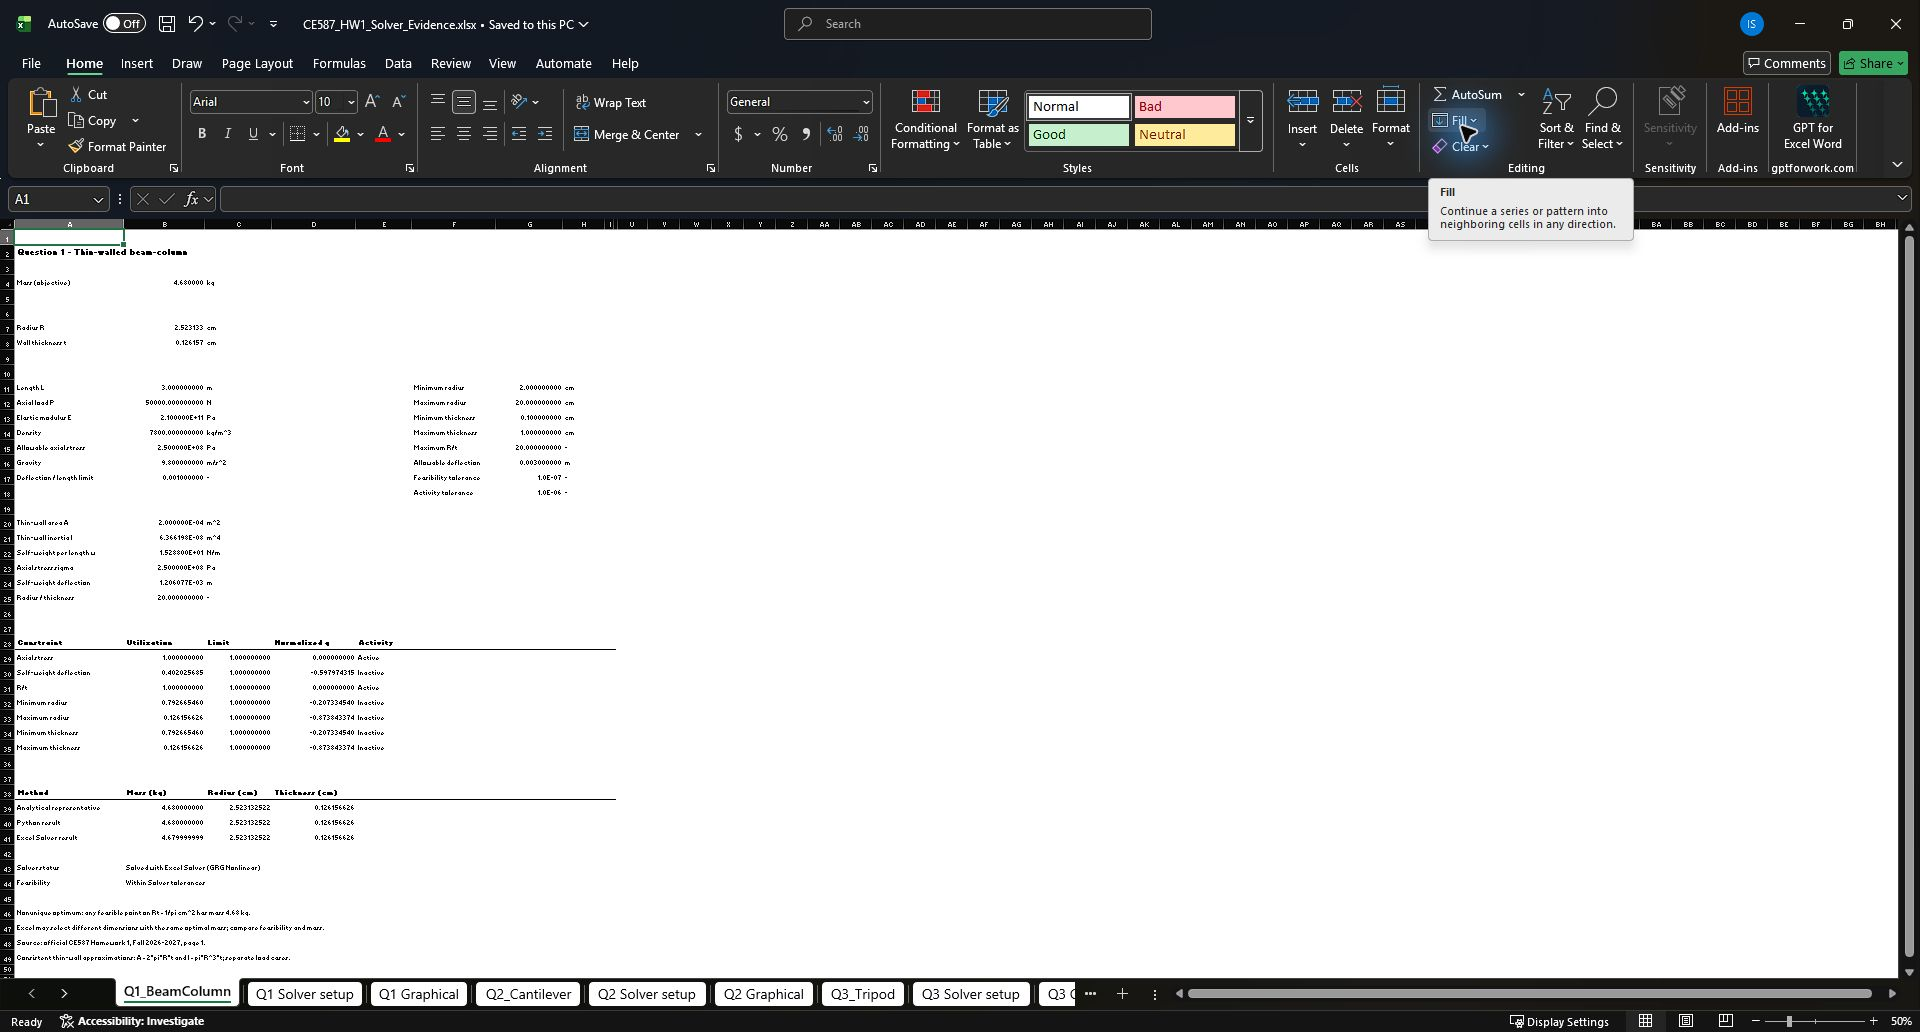
\includegraphics[trim={0 511.5 1140 163.5},clip,width=1.00\textwidth]{report/excel_evidence/Q1_worksheet.jpg}\par\smallskip
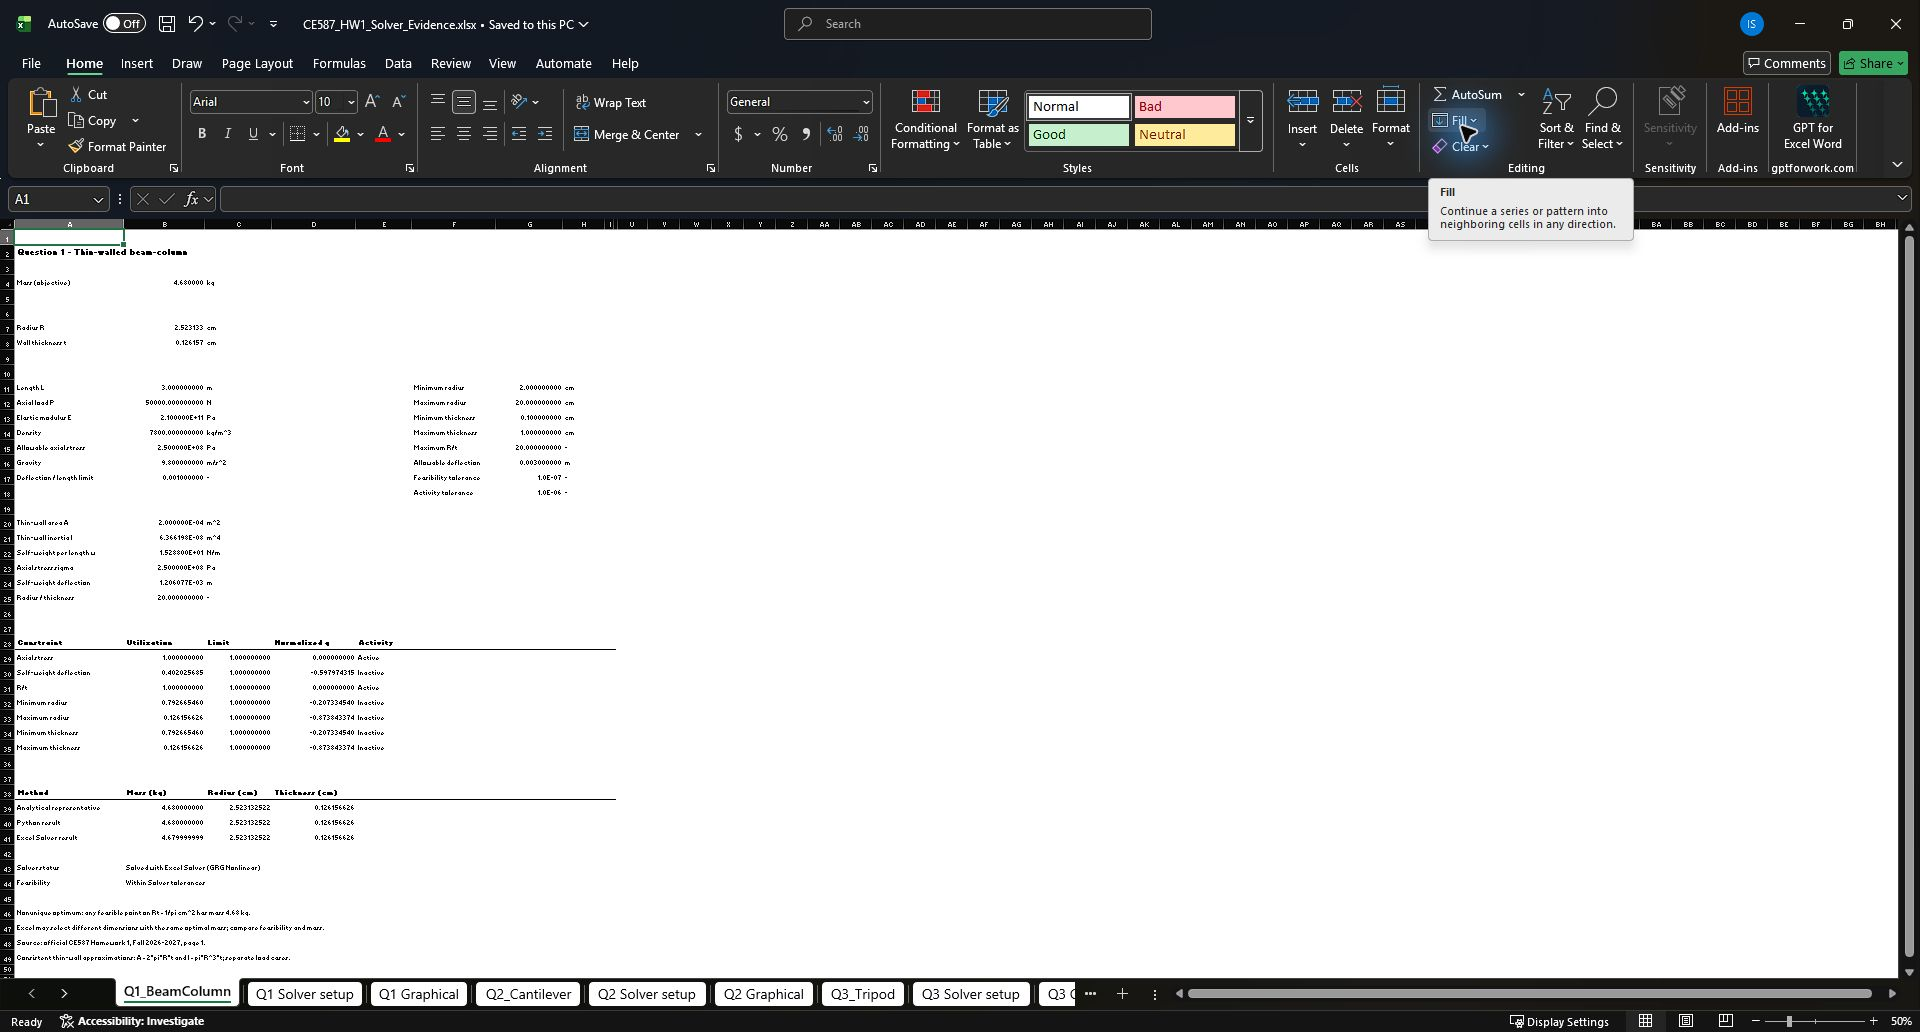
\includegraphics[trim={0 99 1140 472.5},clip,width=1.00\textwidth]{report/excel_evidence/Q1_worksheet.jpg}
\caption{Q1: actual Excel worksheet at the saved design; objective and variables above, constraint checks and results below.}
\end{figure}
\clearpage
\begin{figure}[H]
\centering
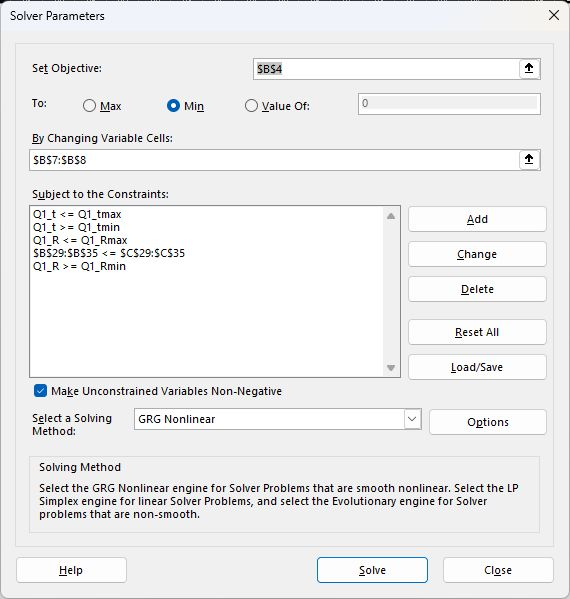
\includegraphics[width=0.83\textwidth,height=0.84\textheight,keepaspectratio]{report/excel_evidence/Q1_solver.jpg}
\caption{Q1: actual Excel Solver Parameters dialog showing the loaded model.}
\end{figure}
\clearpage
\subsection{Question 2}
\begin{figure}[H]
\centering
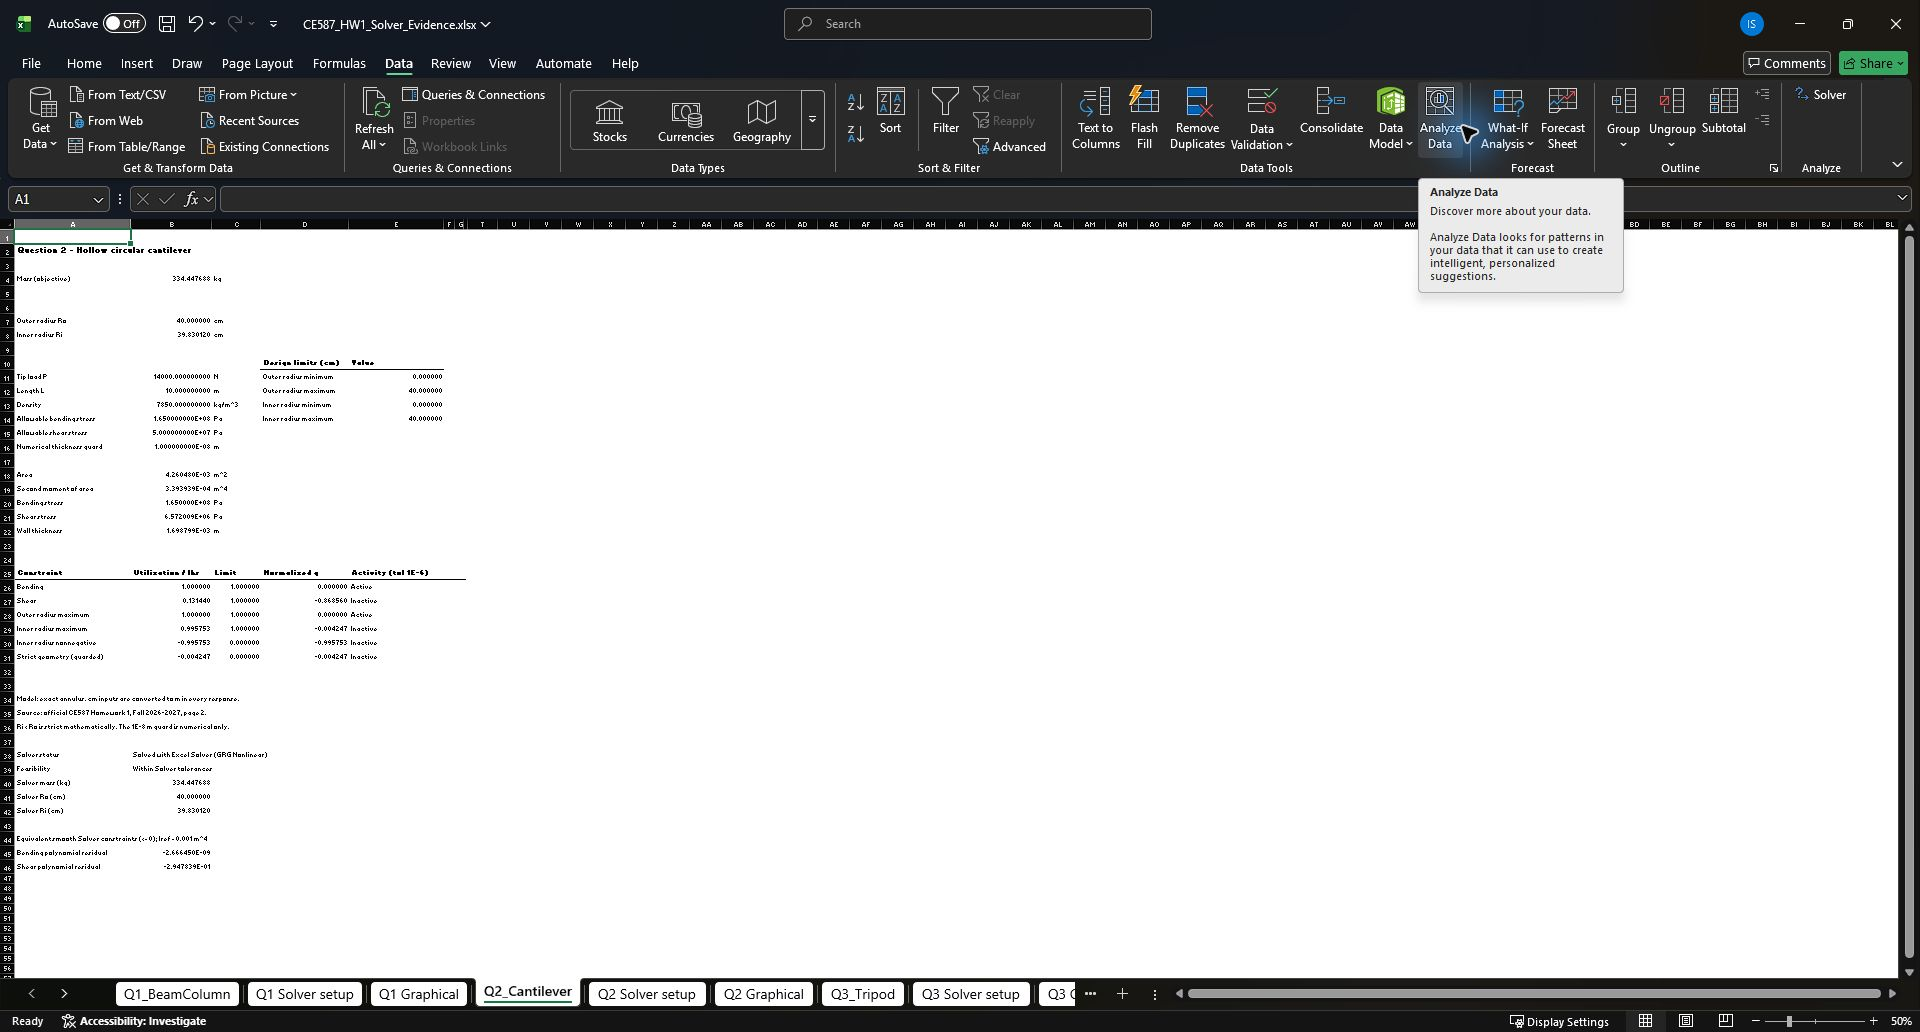
\includegraphics[trim={0 513 1083.75 163.5},clip,width=1.00\textwidth]{report/excel_evidence/Q2_worksheet.jpg}\par\smallskip
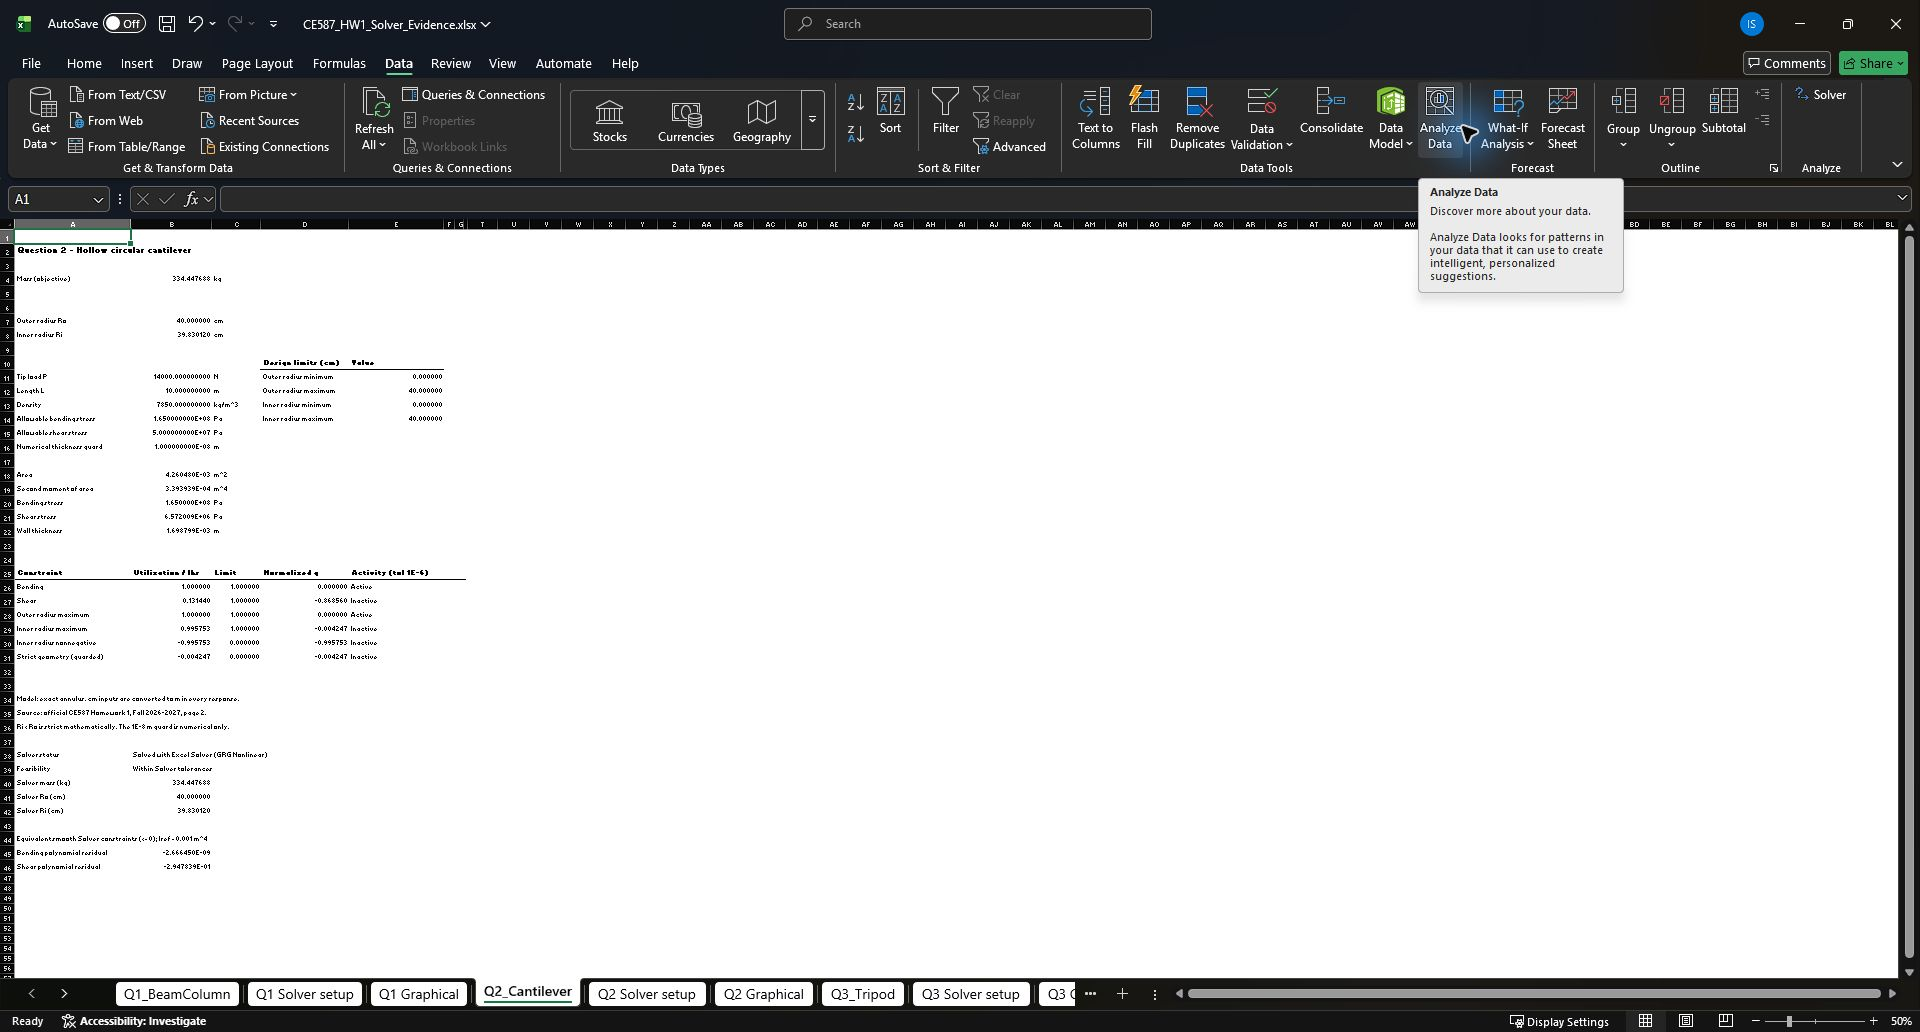
\includegraphics[trim={0 114 1083.75 420},clip,width=1.00\textwidth]{report/excel_evidence/Q2_worksheet.jpg}
\caption{Q2: actual Excel worksheet at the saved design; objective and variables above, constraint checks and results below.}
\end{figure}
\clearpage
\begin{figure}[H]
\centering
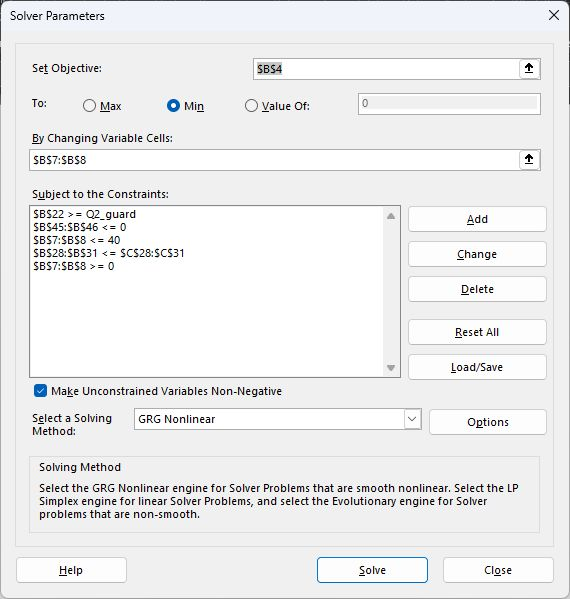
\includegraphics[width=0.83\textwidth,height=0.84\textheight,keepaspectratio]{report/excel_evidence/Q2_solver.jpg}
\caption{Q2: actual Excel Solver Parameters dialog showing the loaded model.}
\end{figure}
\clearpage
\subsection{Question 3}
\begin{figure}[H]
\centering
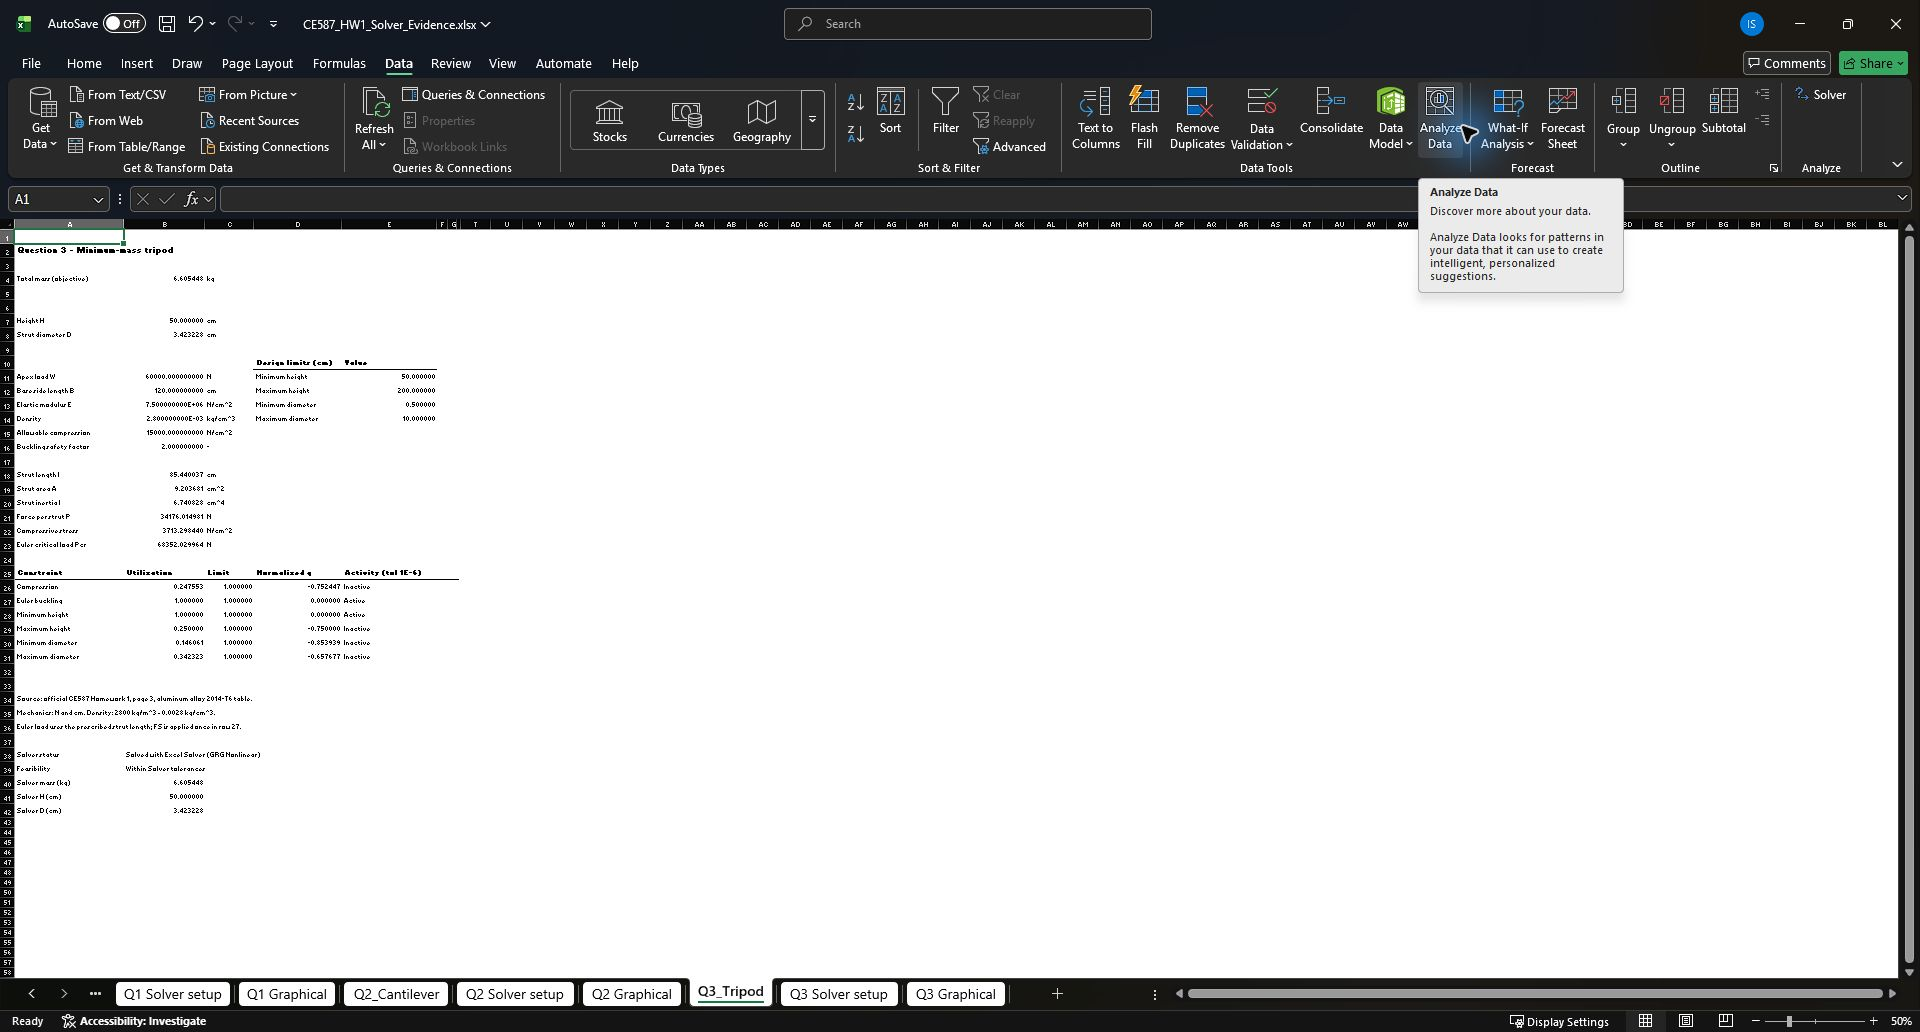
\includegraphics[trim={0 513 1091.25 163.5},clip,width=1.00\textwidth]{report/excel_evidence/Q3_worksheet.jpg}\par\smallskip
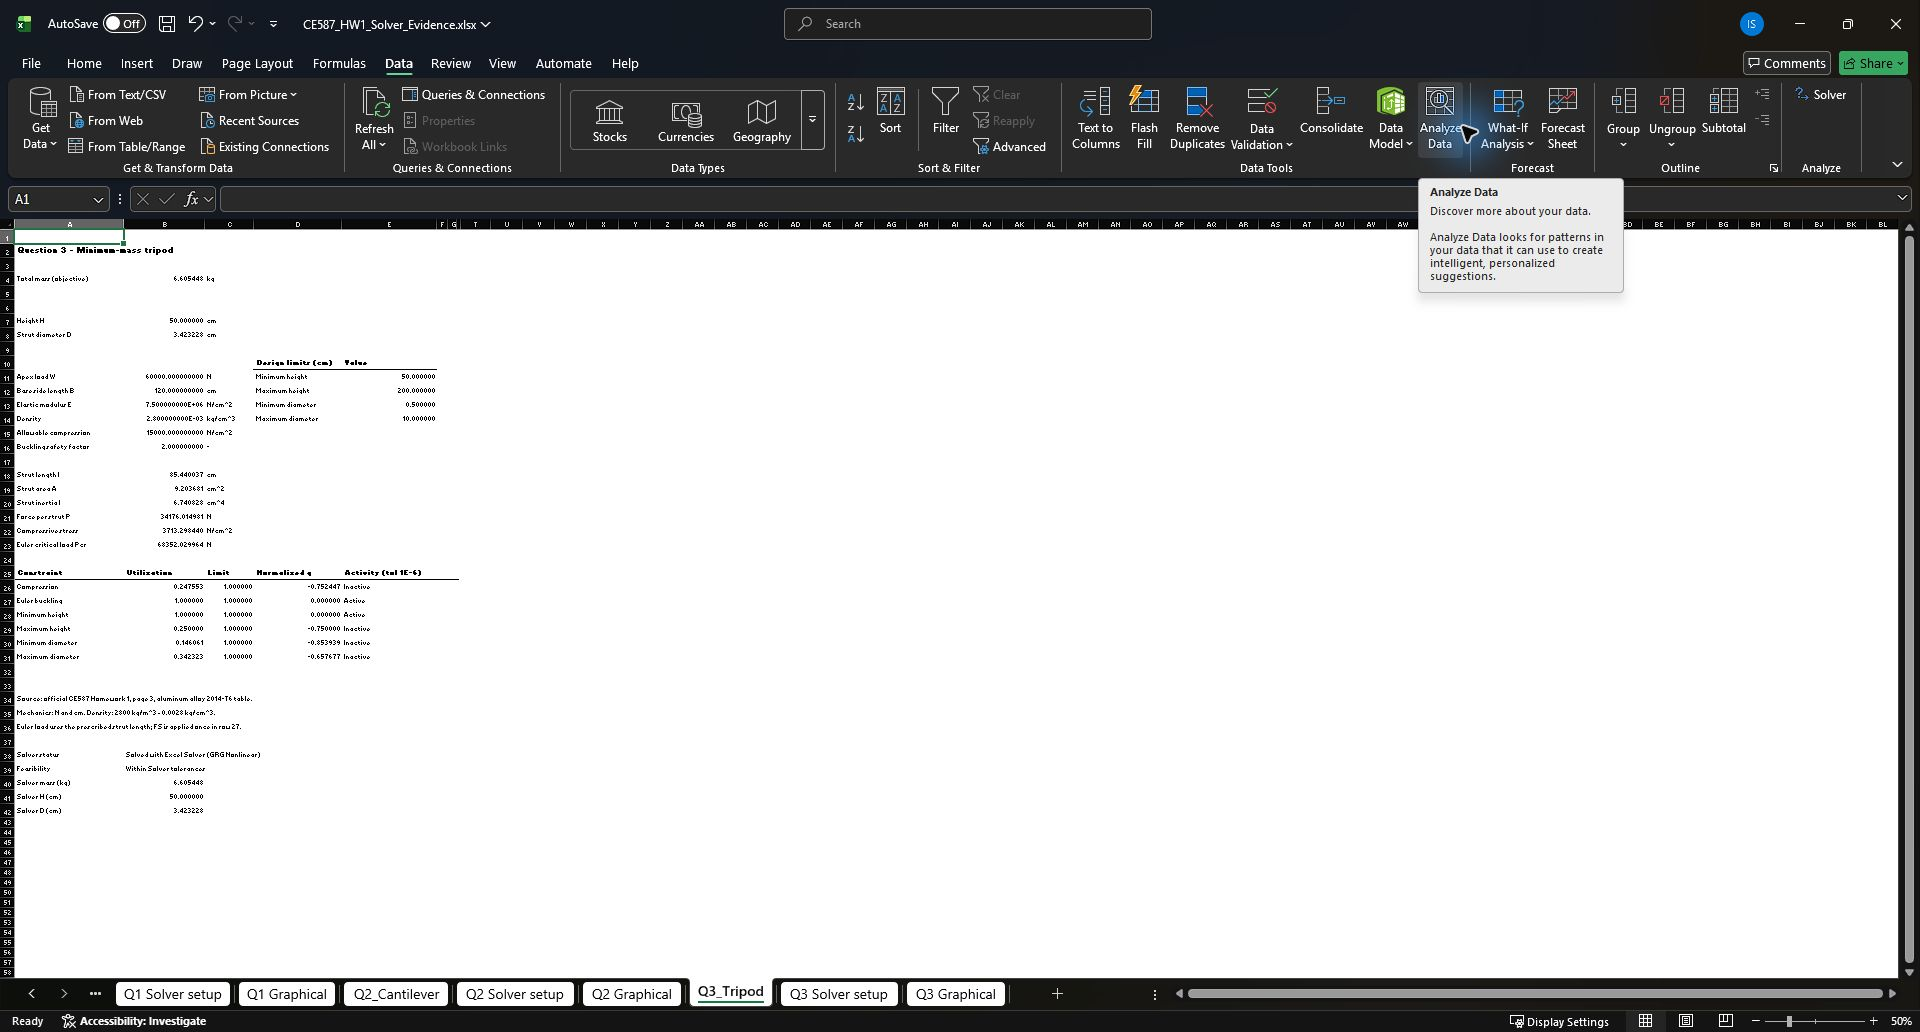
\includegraphics[trim={0 156 1091.25 420},clip,width=1.00\textwidth]{report/excel_evidence/Q3_worksheet.jpg}
\caption{Q3: actual Excel worksheet at the saved design; objective and variables above, constraint checks and results below.}
\end{figure}
\clearpage
\begin{figure}[H]
\centering
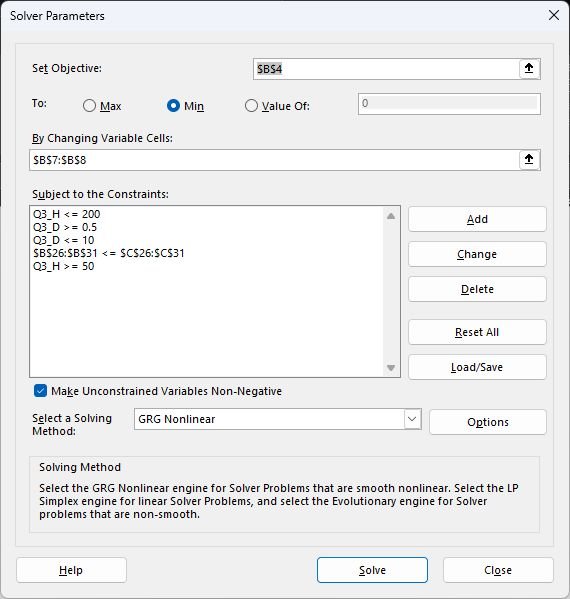
\includegraphics[width=0.83\textwidth,height=0.84\textheight,keepaspectratio]{report/excel_evidence/Q3_solver.jpg}
\caption{Q3: actual Excel Solver Parameters dialog showing the loaded model.}
\end{figure}


\clearpage
\setcounter{figure}{0}
\renewcommand{\thefigure}{B.\arabic{figure}}
\section{Excel Solver check from different starts}\label{app:fresh}
The saved GRG Nonlinear models were run again in Microsoft Excel from the initial designs below. Each run returned ``Solver found a solution. All Constraints and optimality conditions are satisfied.'' The saved design and its mass were reproduced in each case. These numerical checks support the analytical global-optimality arguments in the main solution.

\begin{table}[H]
\centering\small
\caption{Additional Excel Solver runs; all dimensions are in cm.}
\begin{tabular}{@{}lp{0.21\textwidth}p{0.33\textwidth}r@{}}\toprule
Q. & Starting design & Returned design & Mass (kg)\\\midrule
Q1 & $(R,t)=(3,0.15)$ & $(2.52313,0.126157)$ & 4.680000\\
Q2 & $(R_o,R_i)=(30,20)$ & $(40.0000,39.8301)$ & 334.447688\\
Q3 & $(H,D)=(100,5)$ & $(50.0000,3.42323)$ & 6.605448\\
\bottomrule\end{tabular}
\end{table}
The maximum positive normalized residual was $1.46\times10^{-10}$ in Q1, within the Solver precision of $10^{-9}$. Q2 and Q3 satisfied all normalized inequalities. Substitution of the returned dimensions into the independent response calculations confirmed the masses and constraint checks.

\begin{figure}[H]
\centering
\textbf{Q1}\par\smallskip
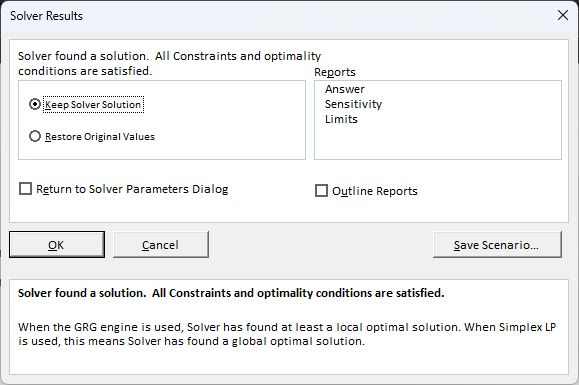
\includegraphics[trim={0 218.25 0 0},clip,width=0.95\textwidth]{verification/fresh_solver/Q1_solver_result.jpg}\par\medskip
\textbf{Q2}\par\smallskip
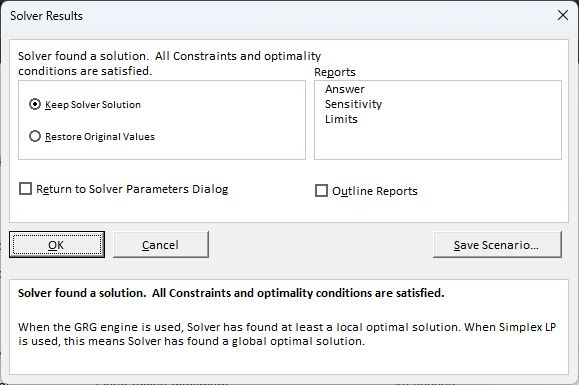
\includegraphics[trim={0 218.25 0 0},clip,width=0.95\textwidth]{verification/fresh_solver/Q2_solver_result.jpg}\par\medskip
\textbf{Q3}\par\smallskip
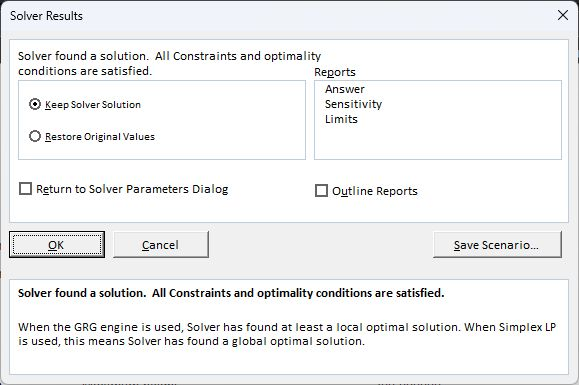
\includegraphics[trim={0 218.25 0 0},clip,width=0.95\textwidth]{verification/fresh_solver/Q3_solver_result.jpg}\par\medskip
\caption{Actual Excel Solver Results messages from the additional runs. Crops show each success message; full dialog captures are retained with the verification files.}
\end{figure}

\end{document}
